% Inbuilt themes in beamer
\documentclass[aspectratio=169]{beamer}
\usepackage{graphicx}
% Theme choice:
\usetheme{CambridgeUS}

% Title page details: 
\title{Chapter 21: Consumer Theory} 
\author{Discussion section 4}
\date{November 2023}

\begin{document}

% Title page
\begin{frame}
    \titlepage 
\end{frame}

% Outline frame
\begin{frame}{Outline}
Remember the core of microeconomics: we all face tradeoffs.

\vspace{2mm}

Consumers have to choose how to allocate limited resources to best satisfy their wants.

\vspace{2mm}

They will do so like good economists, by \textit{thinking at the margin}. 
\end{frame}

% \begin{frame}{Market for coffee}
%     \centering
%     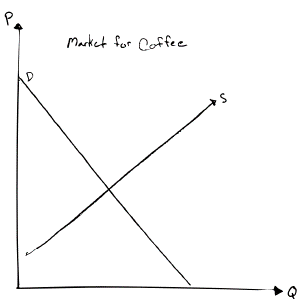
\includegraphics[width = 0.4\textwidth,keepaspectratio]{../figs/coffee1.png}
% \end{frame}

\begin{frame}{Budget constraint}
    Consider two goods: movie tickets and baseball tickets.

    You have \$100 for your monthly entertainment budget. Movie tickets cost \$10, and baseball tickets cost \$20.
    \centering
        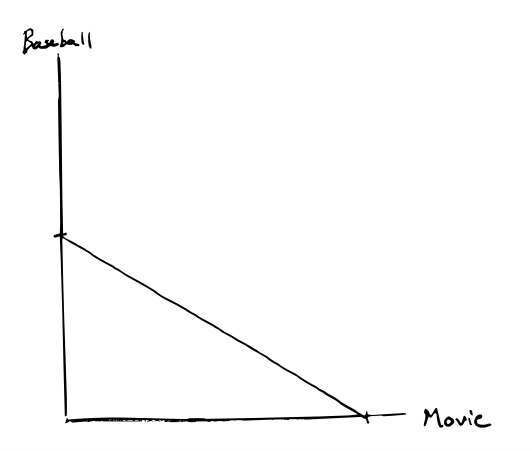
\includegraphics[width = 0.3\textwidth,keepaspectratio]{../figs/BC1.png}
\end{frame}

\begin{frame}{Budget constraint}
    What are the intercepts on the budget constraint?

    \vspace{2mm}

    What is the slope? Does it depend on your budget?

    \centering
        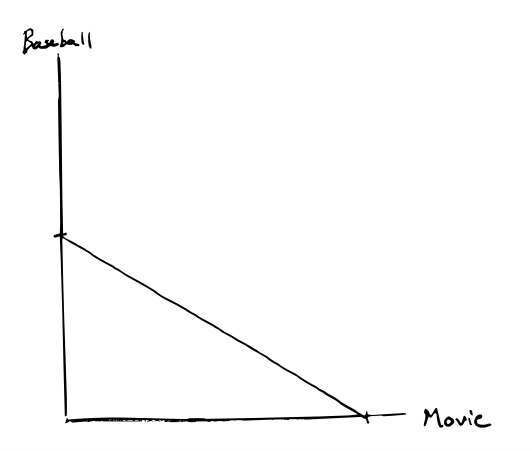
\includegraphics[width = 0.3\textwidth,keepaspectratio]{../figs/BC1.png}
\end{frame}

\begin{frame}{Budget constraint}
    Slope depends on relative price, position depends on total resources
    \centering
        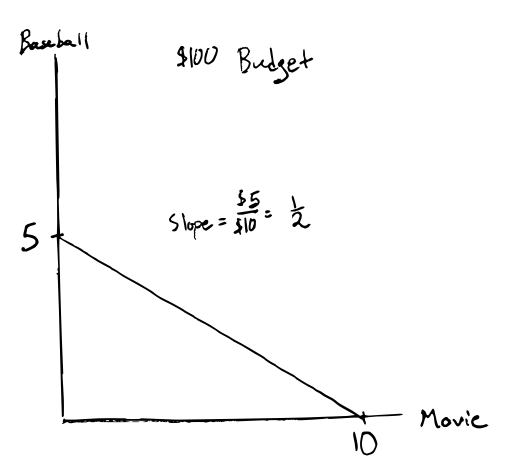
\includegraphics[width = 0.4\textwidth,keepaspectratio]{../figs/BC2.png}
\end{frame}

\begin{frame}{Indifference curves}
    How do we choose among all the different possible consumption points?

    \vspace{2mm}

    We will look at our \textit{indifference curves}.

    \vspace{2mm}

    What does an indifference curve represent?
\end{frame}

\begin{frame}{Indifference curves}
    How do we choose among all the different possible consumption points?

    \vspace{2mm}

    We will look at our \textit{indifference curves}.

    \vspace{2mm}

    What does an indifference curve represent?

    \vspace{2mm}
    \begin{center}
        \textit{All the combinations of goods for which we are equally happy.}
    \end{center}
\end{frame}

\begin{frame}{Principles for ICs}
    \begin{itemize}
        \item Consumers always prefer more
        \item Downward sloping
        \item Do not cross
        \item Inwardly-bowed
    \end{itemize}

    Where does the inwardly-bowed shape come from?
\end{frame}

\begin{frame}{Extreme cases}
    Where does the inwardly-bowed shape come from?

    \vspace{2mm}

    The \textit{marginal rate of substitution} (MRS)

    \vspace{2mm}

    Think about these principles in two extreme cases:
    \begin{itemize}
        \item Perfect substitutes
        \item Perfect complements
    \end{itemize}
\end{frame}

\begin{frame}{Optimal choices}
    How can we combine these two tools to make an optimal choice?
\end{frame}

\begin{frame}{Optimal choices}
    How can we combine these two tools to make an optimal choice?

    \vspace{2mm}

    We want the point on our budget which puts us at the highest indifference curve.

    \vspace{2mm}

    How can we find this?

\end{frame}

\begin{frame}{Optimal choices}
    We want the point on our budget which puts us at the highest indifference curve.

    \vspace{2mm}

    How can we find this?

    \vspace{2mm}

    Equate the \textit{slope} of the BC to the MRS (slope of the IC)

    \vspace{2mm}

    Just what we saw in the free market equilibrium!

\end{frame}

\begin{frame}{Comparative statics}
    We know have a powerful tool for finding optimal choices of consumers

    \vspace{2mm}

    Can we use this to think about the effect of a change in price?
\end{frame}

\begin{frame}{Price increase}
    Suppose this is our budget constraint and optimal choice

    \centering
        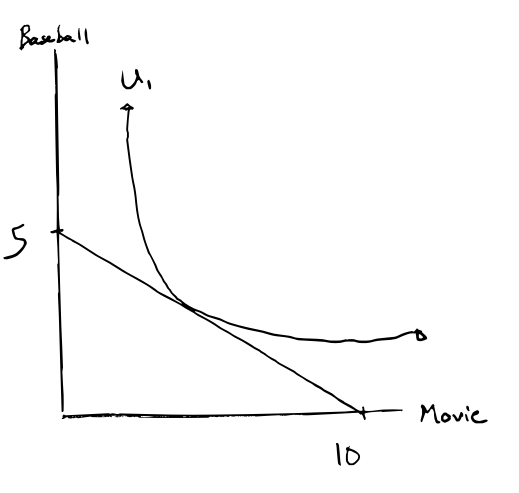
\includegraphics[width = 0.4\textwidth,keepaspectratio]{../figs/OC1.png}

\end{frame}

\begin{frame}{Price increase}
    What happens if the price of baseball tickets falls by 50\%?

\end{frame}

\begin{frame}{Price increase}
    What happens if the price of baseball tickets falls by 50\%?
    \centering
        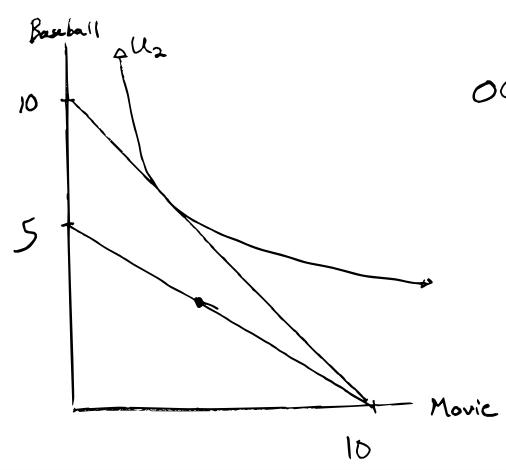
\includegraphics[width = 0.4\textwidth,keepaspectratio]{../figs/OC2.png}
\end{frame}

\begin{frame}{Price increase}
    Was the change unambiguous?

    \vspace{2mm}

    What effects are at play here?
\end{frame}

\begin{frame}{Price increase}
    Was the change unambiguous?

    \vspace{2mm}

    What effects are at play here?
    \begin{itemize}
        \item Income effect
        \item Substitution effect
    \end{itemize}
\end{frame}

\begin{frame}{Income and substitution effects}
    \centering
        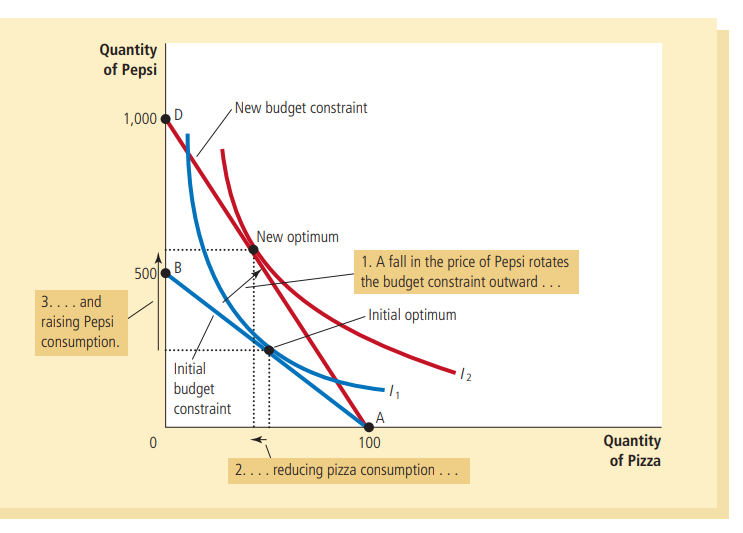
\includegraphics[width = 0.7\textwidth,keepaspectratio]{../figs/effects.png}
\end{frame}

\begin{frame}{Wage increase}
    What is the tradeoff facing workers?

    \vspace{2mm}

    What do they balance in their budget constraint?
\end{frame}

\begin{frame}{Wage increase}
    What is the tradeoff facing workers?  What do they balance in their budget constraint?

    \vspace{2mm}

    Workers balance consumption and leisure time.

    \vspace{2mm}

    What will happen when their wages go up?

\end{frame}

\begin{frame}{Wage increase}
    What will happen when workers' wages go up?

    \vspace{2mm}

    We will see the same two effects as before.
    \begin{itemize}
        \item Income: we are now wealthier, and so we may want to spend some of that wealth on more leisure time.
        \item   Substitution: leisure is now relatively more expensive than consumption (why?), so we may want to increase consumption and decrease leisure.
    \end{itemize}
 
\end{frame}

\begin{frame}{Wage increase}
    Net effect is \textit{ambiguous} --- but labor economists usually think that higher wages lead workers to work more hours. 
\end{frame}

\end{document}